\documentclass[11pt]{article}
\usepackage[preprint]{acl}
\usepackage{times}
\usepackage{latexsym}
\usepackage[T1]{fontenc}
\usepackage[utf8]{inputenc}
\usepackage{microtype}
\usepackage{courier}
\usepackage{graphicx}
\usepackage{booktabs}
\usepackage{amsmath,amssymb}
\usepackage{tabularx}
\usepackage{url}
\newcommand{\adAuc}{0.7725}
\newcommand{\adAp}{0.4217}
\newcommand{\annthyroidAuc}{0.7199}
\newcommand{\annthyroidAp}{0.2034}
\newcommand{\breastwAuc}{0.9840}
\newcommand{\breastwAp}{0.9596}
\newcommand{\pimaAuc}{0.7155}
\newcommand{\pimaAp}{0.5383}
\newcommand{\pageblocksAuc}{0.9143}
\newcommand{\pageblocksAp}{0.5339}
\newcommand{\yeastAuc}{0.3885}
\newcommand{\yeastAp}{0.2903}
\newcommand{\syntheticAuc}{0.9419}
\newcommand{\syntheticAp}{0.7618}
\newcommand{\adAucDiff}{-0.15}
\newcommand{\adApDiff}{-1.63}

\newcommand{\projectrepository}{\textbf{Public GitHub repository URL required before submission.}}

\title{Reproducing and Extending OptIForest for Unsupervised Anomaly Detection}
\author{Surendra Raj Pandey \\ Student ID 60985194 \\ Macquarie University \\ COMP8240 -- Applications of Data Science}
\date{}
\begin{document}
\maketitle
\begin{abstract}
This project reproduces an OptIForest experiment on the supplied AD dataset and extends the evaluation to five existing benchmarks and a constructed synthetic dataset. The final experiments retain the authors' detector implementation, use explicit random seeds, and save per-run scores and metadata. On AD, the reproduced mean ROC-AUC is \adAuc{} and average precision is \adAp{}, compared with published values of 0.774 and 0.438. The extension evaluates Annthyroid, BreastW, Pima, PageBlocks, Yeast and a two-dimensional dataset containing point, boundary and clustered anomalies. A common standardisation procedure is used for the extension following a computationally expensive raw-feature pilot. Conventional Isolation Forest provides a comparison under the same evaluation protocol. Results vary with dataset and anomaly structure, demonstrating the importance of examining weaker outcomes alongside successful cases. An exploratory LLM explanation audit supplements numerical evaluation. The report documents reproducibility decisions, ethical considerations and the limits of generalisation from benchmark and synthetic data.
\end{abstract}

\section{Introduction}
Anomaly detection ranks observations by how unusual they are relative to a dataset. In this project, observations have numerical features and binary benchmark labels, but those labels are withheld from detector fitting. The practical question is whether an existing unsupervised implementation produces useful rankings when the data source and anomaly structure change.

The selected default project is \emph{OptIForest: Optimal Isolation Forest for Anomaly Detection} \citep{xiang2023optiforest}.\footnote{Source paper: \url{https://www.ijcai.org/proceedings/2023/264}.} The method builds on isolation-based detection \citep{liu2008isolation}. Its theoretical analysis motivates an expected branching factor of $e$, and its implementation combines locality-sensitive partitions with clustering-based reconstruction. The source study evaluates 20 datasets with repeated experiments. The present project focuses on the supplied AD dataset and six extension datasets.

Three questions guide the work. First, how closely does executing the original implementation reproduce the published AD scores? Second, how does performance change across additional benchmarks and controlled synthetic anomaly types? Third, what limitations and ethical issues affect interpretation of the resulting rankings and explanations? These questions connect computational reproduction to empirical analysis and responsible reporting.

The project contributes a checked data-conversion pipeline, a documented synthetic generator, a seeded experiment runner, a conventional Isolation Forest comparison, and an exploratory explanation audit. The final report uses saved experimental evidence. Earlier Mac results are retained as a separate progress-stage record so that changes in environment and preprocessing remain traceable.

\section{Replication of Original Work}
\subsection{Original implementation and input}
The supplied \texttt{ad.csv} contains 3,279 observations and 1,555 numerical features. Its final column contains the evaluation label, with 2,820 normal observations and 459 anomalies, giving an anomaly proportion of 14.00\%. The loader reads a headerless CSV, separates the last column, and fits the detector to the feature matrix. Scores are computed for every observation in that same matrix. This evaluates outlier ranking within a fixed dataset.

The model configuration is \texttt{OptIForest('L2OPT', 100, 403, 0)}. The internal sampler draws 512 observations without replacement for each tree. The cut threshold is 403 and the granularity parameter retains its default value of one. The zero branch setting samples two or three branches with probabilities $3-e$ and $e-2$, respectively. Its expected branch count is therefore
\begin{equation}
2(3-e)+3(e-2)=e.
\end{equation}
The implementation uses both NumPy's random generator and Python's \texttt{random} module, so both must be seeded.

The decision function returns more negative values for stronger anomalies. The experimental runner follows the supplied demonstration by negating these values before calculating ranking metrics. Reversing this convention would reverse the scientific interpretation of the scores. The code's internal row indices support tree construction and are appended after the feature matrix has been separated from the evaluation labels.

\subsection{Environment and source verification}
The earlier project update used Python 3.9.6 on the student's Mac. The final rerun uses Python 3.12 in a Linux execution environment. Table~\ref{tab:environment} records the final dependency versions. This distinction matters especially for execution time, which depends on the host and competing processes.

\begin{table}[t]
\centering\small
\begin{tabular}{ll}\toprule
Component & Final environment \\ \midrule
Python & 3.12 \\
NumPy & 1.26.4 \\
pandas & 2.2.3 \\
SciPy & 1.13.1 \\
scikit-learn & 1.6.1 \\
Matplotlib & 3.9.4 \\
\bottomrule\end{tabular}
\caption{Pinned environment for the final experiments and figures. The package includes the full dependency snapshot.}\label{tab:environment}
\end{table}

An initial compatibility check failed under NumPy 2 because the supplied detector calls \texttt{np.mat}. A separate environment pinned to NumPy 1.26.4 resolved that dependency failure. All seven detector Python files were compared byte for byte with the authors' public repository tree \texttt{a8be90d3ba76} (full identifier recorded in the project). They matched. The project repository contains these files with attribution and identifies the experiment and data-processing scripts added for this assessment.\footnote{Project code, results and report source: \projectrepository}

The upstream tests were also examined. Running them from the project root initially exposed working-directory assumptions. After resolving data paths relative to each test file, one fixture still passed 1,556-dimensional indexed centers to a function receiving 1,555-dimensional feature vectors. Removing the fixture's extra index column corrected that mismatch. These changes affect the test harness. Detector source files retain their original bytes. The test output is included with the project.

A runtime warning also occurs when equally sized child partitions give a zero standard deviation in a local statistic. The original code then applies \texttt{min(0.0, NaN)}, which yields zero in this call order. The statistic subsequently selects the ordinary LSH routing path. The final runner records warning counts and checks every returned score for finiteness. This provides evidence about successful execution while preserving visibility of the upstream numerical issue.

\subsection{Replicated results and comparison}
Table~\ref{tab:replication} separates the published result, the progress-stage experiment and the final seeded rerun. Published percentages are converted to the $[0,1]$ scale. The original paper calls its precision--recall summary AUC-PR, whereas the supplied demonstration computes \texttt{average\_precision\_score}. The present report uses \emph{average precision} (AP) for that implementation-specific quantity.

\begin{table}[t]\centering\small
\begin{tabular}{lrr}\toprule
Experiment & ROC-AUC & AP / AUC-PR \\ \midrule
Published & 0.7740 & 0.4380 \\
Earlier Mac run & 0.77434 & 0.43662 \\
Final seeded run & \adAuc & \adAp \\
\bottomrule\end{tabular}
\caption{Mean AD results. Published standard deviations are 0.007 and 0.031. The earlier Mac experiment reported 0.00675 and 0.03863. The earlier Mac run used 15 repetitions. Final variability appears in Table~\ref{tab:results}.}\label{tab:replication}
\end{table}

The final mean differs from the paper by \adAucDiff{} percentage points in ROC-AUC and \adApDiff{} percentage points in the precision--recall summary. This comparison supports reproduction of the AD experiment within the variability of stochastic execution. Original random seeds are unavailable, dependency versions differ, and the reference means are rounded. These factors prevent a claim of exact numerical identity. The wider comparative study across all 20 original datasets is outside the reproduced experimental scope.

\section{Construction of New Data}
\subsection{Existing benchmark datasets}
The five additional benchmarks are supplied in ADBench NPZ format \citep{han2022adbench}.\footnote{Benchmark source: \url{https://github.com/Minqi824/ADBench/tree/main/adbench/datasets/Classical}.} Each archive contains a feature matrix \texttt{X} and an existing binary label vector \texttt{y}. Table~\ref{tab:data} describes the exact representations evaluated here. The underlying source datasets include thyroid measurements, breast cytology features, diabetes-related measurements, document-block features and protein-localisation features.

\begin{table*}[t]\centering\small
\begin{tabular}{lrrrrrl}\toprule
Dataset & Rows & Features & Anomalies & Anomaly rate & Duplicates & Domain \\ \midrule
Annthyroid & 7,200 & 6 & 534 & 7.42\% & 138 & Healthcare \\
BreastW & 683 & 9 & 239 & 34.99\% & 234 & Healthcare \\
Pima & 768 & 8 & 268 & 34.90\% & 0 & Healthcare \\
PageBlocks & 5,393 & 10 & 510 & 9.46\% & 0 & Document analysis \\
Yeast & 1,484 & 8 & 507 & 34.16\% & 31 & Biology \\
Synthetic & 2,000 & 2 & 200 & 10.00\% & 0 & Controlled simulation \\
\bottomrule\end{tabular}
\caption{Extension datasets verified from project files. Duplicates count repeated complete feature-and-label rows beyond the first occurrence. The evaluated benchmark representations may differ from the original source collections.}\label{tab:data}
\end{table*}

Preparation concatenates \texttt{X} with \texttt{y} as the final column and writes a headerless CSV with no index. Validation checks shape, binary labels and finite values. Reading the CSV back must reproduce the NPZ values within a numerical tolerance of $10^{-12}$. All five files passed these checks. File hashes and dataset statistics are saved in \texttt{data\_audit.json}, enabling the evaluated versions to be identified precisely.

Duplicate observations are retained because removing them would alter the supplied benchmark distribution and potentially change the meaning of existing labels. BreastW has 234 repeated rows, a substantial fraction of its small sample. Retaining these observations preserves comparability with the supplied representation, but repeated patterns can influence both tree construction and score ties. Consequently, the effective diversity of this dataset is lower than its row count alone suggests.

Source identity must be distinguished from benchmark identity. For example, the UCI Breast Cancer Wisconsin collection has 699 observations, while the supplied BreastW representation has 683. UCI Page Blocks has 5,473 examples, while the benchmark contains 5,393. The report uses measured benchmark dimensions and cites the underlying sources \citep{uciThyroid,uciBreast,uciPage,uciYeast}. It does not infer undocumented upstream filtering decisions from these count differences. Source links and these distinctions are recorded in the data documentation.

\subsection{Synthetic generation}
The synthetic dataset is a controlled two-dimensional construction. A NumPy generator with seed 42 creates three normal Gaussian clusters, each containing 600 observations. Their means are $(0,0)$, $(5,5)$ and $(-5,5)$. The corresponding covariance matrices are
\begin{align}
\Sigma_1&=\begin{pmatrix}.8&.1\\.1&.8\end{pmatrix},&
\Sigma_2&=\begin{pmatrix}.9&-.1\\-.1&.9\end{pmatrix},\nonumber\\
\Sigma_3&=\begin{pmatrix}.7&0\\0&.7\end{pmatrix}.&&
\end{align}
These distributions provide normal regions with modest differences in spread and orientation.

Eighty point anomalies are drawn uniformly from two distant rectangles, 40 from $[8,12]\times[-8,-4]$ and 40 from $[-12,-8]\times[-8,-4]$. Seventy boundary anomalies are drawn from two Gaussian distributions centred at $(2.7,0)$ and $(2.5,5)$, with 35 observations each. Their covariance matrices are diagonal with entries $(.12,.35)$ and $(.15,.35)$. Fifty clustered anomalies form a compact Gaussian group centred at $(0,9)$ with covariance $.25I$.

Normal observations receive label zero and the three constructed anomaly groups receive label one. These are labels defined by the generation process. Boundary anomalies may overlap geometrically with the tails of a normal distribution, so the label encodes the construction rule even where spatial separation is difficult. The data are shuffled using the same generator, keeping features, labels and group identifiers aligned.

\begin{figure}[t]\centering
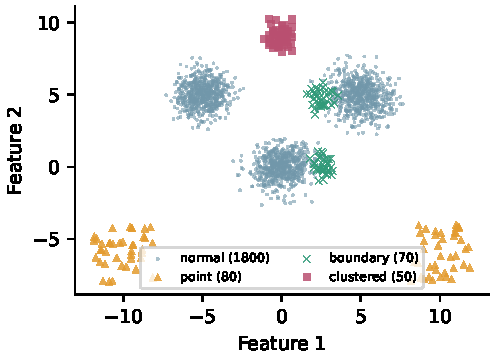
\includegraphics[width=\columnwidth]{figures/synthetic.pdf}
\caption{Constructed dataset in its original coordinates. The final extension experiments standardise these coordinates before model fitting. The distant point groups and overlapping boundary observations create different detection challenges.}\label{fig:synthetic}
\end{figure}

Two output files support different purposes. \texttt{synthetic.csv} contains two feature columns and a binary label for detector evaluation. \texttt{synthetic\_detailed.csv} additionally stores the generating group, enabling subtype analysis. Regenerating the dataset in a separate temporary directory reproduced the stored numerical values within $10^{-12}$. No human annotation was performed, so inter-annotator agreement is inapplicable. The original benchmark labels were reused and synthetic labels were assigned algorithmically.

\subsection{Data snippets and interpretation}
Table~\ref{tab:snippet} shows actual rows from every extension dataset in original units. The complete files and preparation scripts retain full precision. Similar headerless structure is used for every benchmark, with the final field reserved for evaluation labels. Feature columns alone are passed to the detector. The detailed anomaly-type field is used only in subsequent diagnostic analysis.
\begin{table}[t]\centering\small
\begin{tabular}{lrrr}\toprule
Dataset & $x_1$ & $x_2$ & Label \\ \midrule
Annthyroid & 0.73 & 0.0006 & 0 \\
Breastw & 5 & 1 & 0 \\
Pima & 6 & 148 & 1 \\
Pageblocks & 5 & 7 & 0 \\
Yeast & 0.5818 & 0.8882 & 0 \\
Synthetic & -8.807 & -5.729 & 1 \\
\bottomrule\end{tabular}
\caption{First row of each extension CSV in original units. The first two features and final label are displayed. Additional feature columns are omitted for space.}\label{tab:snippet}
\end{table}


\section{Evaluation Methodology}
\subsection{Ranking metrics}
ROC-AUC measures how often an anomalous observation receives a higher score than a normal observation, with half credit for ties. For anomaly set $A$, normal set $N$ and anomaly score $s$, the empirical statistic is
\begin{equation}
\frac{\sum_{a\in A}\sum_{n\in N}[\mathbf{1}(s_a>s_n)+\frac12\mathbf{1}(s_a=s_n)]}{|A||N|}.
\end{equation}
This statistic considers ranking across thresholds. A value near 0.5 represents approximately random ordering. ROC-AUC below 0.5 is retained and examined as a weak ranking under the chosen label convention.

Average precision summarises precision at successive increases in recall,
\begin{equation}
\mathrm{AP}=\sum_k (R_k-R_{k-1})P_k.
\end{equation}
The implementation uses scikit-learn's non-interpolated AP \citep{sklearnap}. It differs from trapezoidal integration of a precision--recall curve. The distinction is relevant because the earlier slides used the shorter label PR-AUC for this calculation. The metric name is corrected here while preserving the underlying computation.

The positive-class prevalence provides a useful reference level for precision--recall interpretation. It is 7.42\% in Annthyroid and 34.99\% in BreastW, so their AP scores have different baseline contexts. Comparing detectors within each dataset avoids attributing every cross-dataset AP difference to detection quality. ROC-AUC and AP are therefore reported together.

\subsection{Final protocol and preprocessing change}
AD retains the supplied numerical representation for replication. For every extension dataset, the final protocol applies \texttt{StandardScaler} to each feature before fitting either detector. Each feature is centred by its dataset mean and divided by its dataset standard deviation. Labels and anomaly-type identifiers are excluded from this transformation.

This decision followed the raw-feature pilot. Some raw datasets completed readily, whereas Pima and PageBlocks failed to finish an initial 100-tree run during several minutes of observed execution. The combination of heterogeneous feature scales, fixed-width LSH bins and exhaustive hierarchical merging makes scale a plausible computational factor. A common standardisation procedure was therefore adopted for all extension datasets. This was a practical decision made during the project, rather than a preregistered protocol or a per-dataset search for the highest label-based score. Completed pilot results and the interruption note are retained.

Both models fit and score the same full dataset. Standardisation also uses that full feature matrix. This protocol evaluates transductive outlier detection, in which the observations to be ranked are already available at fitting time. A deployment study on future observations would require separate fitting and evaluation samples and would fit preprocessing on the training features alone. The current results address the fixed-dataset question.

The smaller extension datasets use 15 runs with seeds 42--56. The larger Annthyroid and PageBlocks conditions use at least three runs, and the independent AD rerun uses at least five. Table~\ref{tab:results} gives the exact completed counts. These unequal budgets reflect observed computation costs and limit the precision of comparisons for the larger datasets. A fresh model is constructed for each seed. The comparison uses scikit-learn Isolation Forest with 100 trees, \texttt{max\_samples=512}, \texttt{contamination='auto'} and one worker. These matching tree and sample budgets support a practical comparison. The implementations have different partitioning and scoring procedures, so this is a baseline comparison under a common data protocol.

The runner saves each completed seed immediately, including ROC-AUC, AP, fitting time, scoring time and warning count. It also saves all scores and labels and records dependency versions, preprocessing and data hashes. Mean scores and population standard deviations use the same divisor convention as the supplied demonstration. Their variation describes model randomness on fixed data. It does not measure uncertainty over newly sampled populations.

Several datasets were processed concurrently on the shared Linux host, with numerical library thread counts limited to one per process. Wall-clock measurements are retained as operational records. They are unsuitable for controlled efficiency comparisons with the earlier Mac experiment or the paper's hardware. The principal comparative evidence is ranking performance.

\subsection{LLM-as-judge explanation audit}
The proposal's LLM component was implemented as a small exploratory audit of explanation quality. Six synthetic observations were sampled with seed 123, using two from each anomaly group. Each received a grounded numerical summary and a deliberately corrupted counterpart, giving 12 explanations. The evidence includes coordinates, nearest generating reference centre, Euclidean distance, raw-pilot model score and score percentile from synthetic seed 42.

The grounded template reports the distance and percentile and limits its claims to position and ranking. The corrupted template replaces the measured distance with zero and asserts certain financial fraud and causal knowledge. These claims provide a controlled test of numerical contradiction and unsupported domain interpretation. Generating centres are explicitly identified as reference information, because they differ from the detector's learned internal structures.

The judge scores four dimensions from one to five. \emph{Faithfulness} assesses agreement with the evidence. \emph{Clarity} assesses how readily the text can be understood. \emph{Calibration} assesses whether certainty and causal claims are warranted. \emph{Usefulness} assesses whether the interpretation helps rather than misleads. The prompt explicitly allows a fluent false explanation to score highly for clarity and poorly for faithfulness. Exact inputs, rubric, scores and reasons are saved.

Judgments were made in one pass by the ChatGPT/Codex assistant during report preparation. The same assistant helped construct the templates, making this an unblinded self-audit. The precise deployed model identifier, temperature and a model snapshot were unavailable. There were no independent human raters and no inter-rater agreement estimate. This component supplies a documented demonstration of the proposed evaluation idea. Its reliability on subtle errors and naturally generated explanations remains unestablished.

\section{Results on New Data}
\begin{table*}[t]\centering\small
\begin{tabular}{lrrrrr}\toprule
Dataset & Runs & OptIForest ROC-AUC & iForest ROC-AUC & OptIForest AP & iForest AP \\ \midrule
AD & 9 & 0.7725 $\pm$ 0.0065 & 0.6918 $\pm$ 0.0181 & 0.4217 $\pm$ 0.0365 & 0.4283 $\pm$ 0.0510 \\
Annthyroid & 5 & 0.7199 $\pm$ 0.0028 & 0.8058 $\pm$ 0.0141 & 0.2034 $\pm$ 0.0078 & 0.2893 $\pm$ 0.0203 \\
BreastW & 15 & 0.9840 $\pm$ 0.0011 & 0.9822 $\pm$ 0.0014 & 0.9596 $\pm$ 0.0044 & 0.9543 $\pm$ 0.0050 \\
Pima & 15 & 0.7155 $\pm$ 0.0037 & 0.6642 $\pm$ 0.0088 & 0.5383 $\pm$ 0.0051 & 0.4926 $\pm$ 0.0093 \\
PageBlocks & 7 & 0.9143 $\pm$ 0.0022 & 0.8994 $\pm$ 0.0091 & 0.5339 $\pm$ 0.0094 & 0.4805 $\pm$ 0.0214 \\
Yeast & 15 & 0.3885 $\pm$ 0.0034 & 0.3965 $\pm$ 0.0078 & 0.2903 $\pm$ 0.0020 & 0.3028 $\pm$ 0.0032 \\
Synthetic & 15 & 0.9419 $\pm$ 0.0248 & 0.9338 $\pm$ 0.0077 & 0.7618 $\pm$ 0.0318 & 0.7587 $\pm$ 0.0129 \\
\bottomrule\end{tabular}
\caption{Final seeded evaluation. AD uses its supplied representation. Extension features are standardised. Values are means $\pm$ population standard deviations. Seeds are consecutive from 42, with the exact number of runs shown. AP is average precision. Both models use 100 trees and samples of 512 observations.}\label{tab:results}
\end{table*}

\begin{figure*}[t]\centering
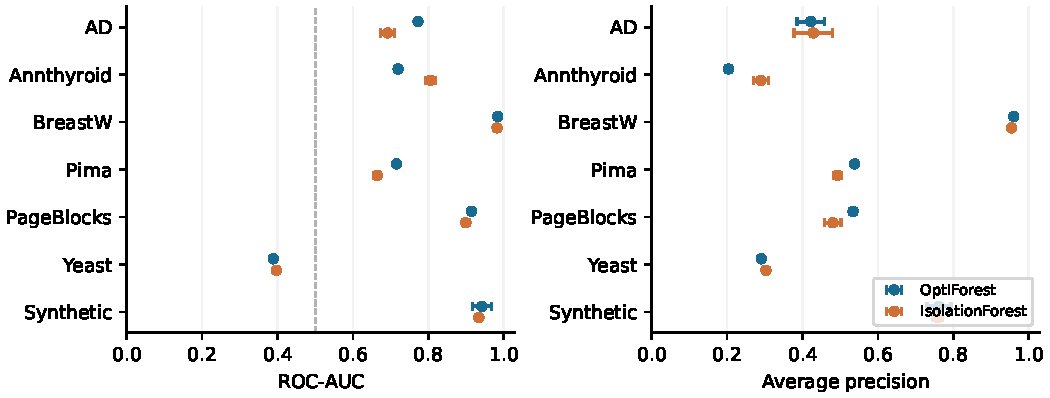
\includegraphics[width=.94\textwidth]{figures/performance.pdf}
\caption{Final mean ranking performance with one standard deviation across seeds. AD uses its supplied representation and extension datasets use standardised features. Cross-dataset AP comparisons also depend on anomaly prevalence.}\label{fig:performance}
\end{figure*}
The nine paired AD reruns place OptIForest's mean ROC-AUC at \adAuc{} (population SD 0.0065) and AP at \adAp{} (SD 0.0365). The paper reports 0.774 and 0.438, respectively, so the final rerun is close in ROC-AUC and lower in AP. The progress-stage Mac run was 0.7743 ROC-AUC and 0.4366 AP over 15 repetitions. Its near match in AP is reassuring, but its sample size, Python version, host and random-state handling differ from this rerun. The nine-run result therefore supports approximate replication of the supplied AD experiment, not exact reproduction of the paper's 20-dataset protocol. The paper's precision--recall summary and this report's non-interpolated AP also need not be identical quantities.

The extension does not show one detector winning everywhere. On standardised Annthyroid, Isolation Forest leads by about 0.086 ROC-AUC and 0.086 AP; both methods rank anomalies above the prevalence baseline, but the benchmark remains difficult. On BreastW, OptIForest has a small advantage of about 0.0019 ROC-AUC and 0.0053 AP. That result should be read with the benchmark's 234 duplicate rows in mind. On Pima, OptIForest leads by about 0.051 ROC-AUC and 0.046 AP. On PageBlocks, it leads by about 0.015 ROC-AUC and 0.053 AP. Yeast is a weak case for both methods: ROC-AUC is below 0.5 and AP is below its 34.2\% anomaly prevalence. We retain the stated score orientation and report this result as a failure case rather than reversing scores after seeing labels.

The synthetic benchmark shows high aggregate ranking performance for both methods, with OptIForest slightly ahead in ROC-AUC (0.9419 versus 0.9338) and effectively tied in AP (0.7618 versus 0.7587). The subtype diagnostic gives a more qualified picture: among the 200 highest-scoring points, both methods recover all point anomalies and nearly all clustered anomalies, but OptIForest selects 8.1\% of boundary anomalies compared with 1.3\% for Isolation Forest. This controlled example suggests that aggregate scores can conceal structural differences. It does not establish that either detector will behave similarly on naturally occurring anomalies. The synthetic distribution is simple and deliberately specified; the labels are construction categories rather than evidence about a real population.

The feature scaling decision also affects interpretation. A short raw-feature pilot gave much weaker results on Annthyroid than the standardised reruns, and raw and standardised synthetic performance differed. The final protocol applies the same StandardScaler transformation to every extension dataset and both detectors, while retaining AD in its supplied representation. Scaling was adopted after a practical runtime problem, not chosen by a search over test performance. The comparison is consequently transparent but not a controlled estimate of the causal effect of scaling: the raw pilot was incomplete, and repeated-run budgets differ across datasets. Future work should preregister both preprocessing conditions and run paired seeds for the full benchmark suite.

Runtime is especially uneven for OptIForest because its hierarchical clustering and LSH operations scale differently across data size, feature scale and duplicate structure. Table~\ref{tab:runtime} therefore reports measured times for reproducibility but they are not treated as a stable cross-machine efficiency ranking. The AD and Annthyroid scoring times were particularly high on this shared host. Across all completed runs, numerical warnings occurred frequently in the unchanged OptIForest implementation, although the saved score arrays were finite. This does not prove numerical stability for other data or environments; it identifies a concrete issue for upstream investigation.

Finally, the exploratory LLM audit is evidence about the evaluation procedure, not about general judge accuracy. It distinguished six deliberately clear synthetic explanations from six fabricated explanations with explicit contradictions, under a rubric that separately scores faithfulness, clarity, calibration and usefulness. The one-pass, unblinded self-audit and absent independent raters prevent an agreement or validity claim. The result motivates a stronger follow-up with held-out explanations, multiple blinded judges and human adjudication of disagreements.


\subsection{Anomaly structure and threshold diagnostics}
The synthetic group identifiers permit a diagnostic beyond aggregate scores. For each seed, the 200 highest anomaly scores are flagged, matching the known 10\% construction prevalence. Table~\ref{tab:subtypes} reports the fraction selected in each group. The choice is a retrospective diagnostic using known simulated prevalence, and is separate from fitting or threshold-free ranking evaluation. Stable row order resolves any tied scores at the cutoff.
\begin{table}[t]\centering\small
\begin{tabular}{lrr}\toprule
Group & OptIForest & iForest \\ \midrule
Point & 100.0\% & 100.0\% \\
Boundary & 8.1\% & 1.3\% \\
Clustered & 99.5\% & 100.0\% \\
Normal & 3.6\% & 3.8\% \\
\bottomrule\end{tabular}
\caption{Mean fraction flagged in each synthetic group when the 200 highest-scoring records are selected. For anomaly groups this is recall. For normal records it is the false-positive rate.}\label{tab:subtypes}
\end{table}


A clustered group can be far from normal centres while containing many nearby members. Isolation therefore depends on how the forest separates that group and its members. Boundary observations are harder because they overlap the edges of normal regions. These mechanisms are hypotheses consistent with the construction. The subtype rates provide the measured evidence. The simulation contains only one fixed mixture and anomaly prevalence, so the experiment does not cover every form of contextual or collective anomaly.

\begin{figure*}[t]\centering
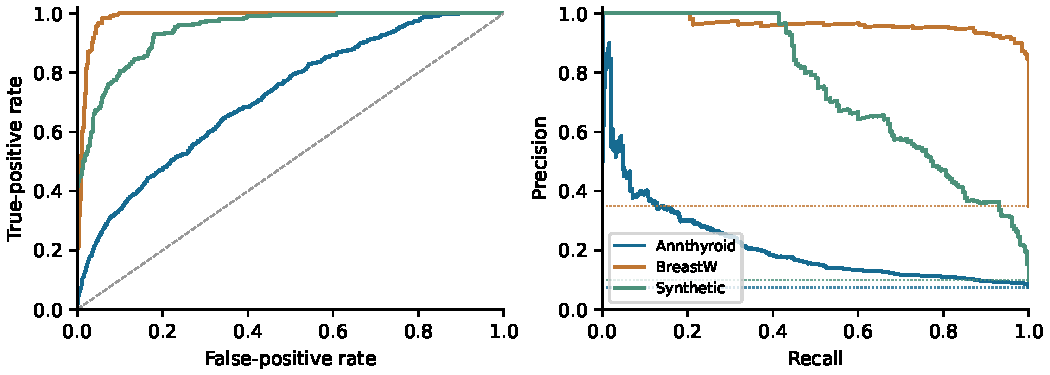
\includegraphics[width=.93\textwidth]{figures/curves.pdf}
\caption{Seed-42 OptIForest ROC and precision--recall curves for three extension datasets. Dotted horizontal lines in the precision--recall panel mark each dataset's anomaly prevalence. Aggregate conclusions use every completed final seed listed in Table~\ref{tab:results}.}\label{fig:curves}
\end{figure*}

\subsection{Explanation audit outcomes}
All six grounded summaries received faithfulness and calibration scores of five and clarity and usefulness scores of four. The six corrupted summaries received faithfulness, calibration and usefulness scores of one, while clarity remained four. Thus the audit separated comprehensible writing from evidence-supported interpretation for these deliberately simple contrasts.

The perfect separation is limited evidence. The pairs use repeated templates, the contradictions are conspicuous, and template construction and judging share an assistant. The results establish that the recorded rubric can be applied to these examples. They provide no estimate of independent judge accuracy, human agreement or performance on subtle hallucinations. In particular, favourable language judgments do not explain why OptIForest produced a score and cannot replace ROC-AUC or AP.

\section{Ethical Considerations}
\subsection{Original work and affected stakeholders}
The original paper motivates anomaly detection in cybersecurity, financial risk and health monitoring. In such settings, false positives can trigger intrusive investigation or unnecessary intervention, while false negatives can leave important events undetected. The proceedings version inspected contains no dedicated ethics section. Ethical scrutiny is therefore needed when interpreting or extending its benchmark findings.

This project treats anomaly labels as operational benchmark targets. A high score records statistical unusualness under a modelling procedure. Using such a score for clinical or financial action would require domain validation, an appropriate threshold and accountable human decision-making. People represented in healthcare data and people subject to later decisions have interests extending beyond a numerical performance improvement. The weak results are consequently as important to report as the strongest cases.

\subsection{Provenance, privacy and permission}
The project reuses supplied ADBench representations and records both their immediate source and identifiable underlying UCI datasets. The current UCI entries for Thyroid Disease, Breast Cancer Wisconsin, Page Blocks and Yeast state CC BY 4.0 terms. ADBench's software repository uses a BSD-2-Clause licence. These facts concern specific sources and do not establish blanket permission for every historical derivative or for unrelated code. The precise upstream transformation history and consent documentation of the Pima benchmark were not recovered. The data documentation records that gap. Broader publication would require resolving applicable permissions and institutional requirements.

Public access alone establishes neither the participants' original consent nor an absence of re-identification risk. This project uses numerical benchmark files without adding identifying fields, and the workflow performs no linkage to external personal records. The explanation audit uses synthetic coordinates exclusively, reducing disclosure risk in LLM inputs. A publishable extension should retain the same data-minimisation principle and verify governance before using newly collected health records.

Pima's historical association with an Indigenous population also warrants care in describing results. Performance on this benchmark should not be generalised to an ethnic group or treated as evidence about inherent group characteristics. The dataset's limited population context and the project's operational anomaly mapping constrain the conclusions.

\subsection{Fairness, transparency and research integrity}
Demographic subgroup fairness was not assessed. The supplied benchmark matrices provide neither an established fairness protocol nor sufficient verified demographic context for that claim. Aggregate AUC and AP can conceal unequal errors across groups. A future applied study would need context-appropriate subgroup evaluation and consultation with relevant stakeholders, alongside protection of sensitive attributes.

The Australian Code for the Responsible Conduct of Research emphasises honesty, rigour, transparency and accountability \citep{nhmrc2018code}. Here these principles are operationalised by retaining weak rankings, recording the preprocessing change, distinguishing progress-stage evidence from final experiments, and saving per-seed outputs and data hashes. Attribution identifies the original algorithm authors, benchmark maintainers and source-data creators. These practices allow the reported computations and methodological decisions to be checked.

Work on ethics sections examines benefits, harms and affected groups \citep{benotti2022ethics}, and EthiCon documents ethical concerns across ACL publications \citep{karamolegkou2025ethicon}. Applying that perspective here links each concern to a concrete choice, such as synthetic-only LLM inputs, restrained clinical interpretation and disclosure of incomplete provenance. An ethics statement cannot itself resolve those empirical or governance limitations.

\subsection{LLM use and disclosure}
Generative AI assisted code preparation, experimental orchestration, analysis and report drafting. The explanation judgments were also recorded by that assistant, which creates an evaluation dependency. The model identity and configuration limitations are disclosed with the audit. Releasing prompts and judgments supports inspection of what occurred, while an independent model and human assessment would be needed to evaluate judge reliability. The student author remains responsible for checking the report, references, code and claims before submission.

\section{Conclusions and Reflections}
The project executed the original detector on AD and compared its scores directly with the published values. The final seeded ROC-AUC of \adAuc{} and AP of \adAp{} provide a concrete reproduction result with documented environmental differences. The extension broadened evaluation to five existing benchmarks and a reproducible synthetic mixture, using a common standardisation procedure and a conventional Isolation Forest comparator.

The project demonstrates that successful execution and transfer across datasets are separate empirical questions. Variation in scale, duplicate patterns, anomaly prevalence and anomaly structure can affect interpretation. Reporting all evaluated datasets and retaining the raw pilot makes these limits visible. A focused follow-up would investigate feature scaling on fixed data, duplicate-sensitive evaluation, and additional independently generated synthetic mixtures with several contamination levels.

The LLM component implemented an exploratory explanation audit with recorded evidence and rubric-based judgments. Its small, unblinded design leaves independent validity unresolved. More rigorous work would separate explanation construction from judging, include subtle errors, use a fixed model configuration and obtain independent human ratings. Together, the numerical and explanation evaluations support a bounded conclusion about this implementation under the recorded experimental conditions.

\clearpage
\bibliography{references}
\clearpage
\appendix
\section{Execution and Evidence Guide}
The project archive includes detector source, original and extension data, the synthetic generator, conversion and validation scripts, experiment outputs and report sources. The dependency pins are in \texttt{requirements.txt}. The full environment snapshot is stored with the results. Paths in the final runner resolve relative to its own source file, so the runner can be invoked from any working directory.

After creating a Python environment and installing the requirements, validate the files with \texttt{python scripts/prepare\_data.py}. Run AD with \texttt{python scripts/run\_final.py --dataset ad}. For an extension, add \texttt{--standardize}, for example \texttt{python scripts/run\_final.py --dataset annthyroid --standardize}. The default is 15 runs. Completed seeds are resumed from disk only when dataset and environment metadata match. Saved score arrays permit figures and metrics to be checked without repeating the expensive detector execution.

Generate the report tables and figures with \texttt{python scripts/build\_results.py}. The command checks the documented minimum run counts, consecutive seeds from 42, and matching model counts within each dataset. Compile \texttt{report/main.tex} using \texttt{latexmk -pdf main.tex} from the report directory. The ACL style and bibliography files are included. The repository URL is stored separately in \texttt{report/repository.tex}.

The main evidence files are \texttt{results/ad\_runs.csv} for AD and the per-dataset CSVs under \texttt{results\_scaled/} for the extensions. Score arrays share the dataset, model and seed in their filenames. Data checks, source hashes, synthetic regeneration and test output are stored under \texttt{results/}. The exact LLM evidence, rubric, judgments and execution disclosure are in \texttt{results/judge/}.

\begin{table}[t]\centering\small
\begin{tabular}{lrrr}\toprule
Dataset & Runs & Fit (s) & Score (s) \\ \midrule
AD & 9 & 54.00 & 117.79 \\
Annthyroid & 5 & 21.90 & 162.44 \\
BreastW & 15 & 15.74 & 18.05 \\
Pima & 15 & 21.14 & 20.38 \\
PageBlocks & 7 & 15.44 & 124.32 \\
Yeast & 15 & 16.89 & 36.24 \\
Synthetic & 15 & 12.53 & 37.68 \\
\bottomrule\end{tabular}
\caption{Mean OptIForest wall time per run on the shared evaluation host. Times are environment-specific and are not directly compared with the earlier Mac run.}\label{tab:runtime}
\end{table}



\section{Data Sources and Representation Notes}
The original AD CSV is supplied with the authors' OptIForest repository. The project evaluates its exact numerical representation. The five new existing datasets come from the supplied ADBench archives, named \texttt{2\_annthyroid.npz}, \texttt{4\_breastw.npz}, \texttt{29\_Pima.npz}, \texttt{27\_PageBlocks.npz} and \texttt{47\_yeast.npz}. The source and permission notes in \texttt{DATA\_SOURCES.md} distinguish software licences from dataset terms. The retained archives support verification of conversion without relying on a potentially changing upstream download.

\section{Example LLM Audit Pair}
For synthetic row 118, the evidence contains coordinates $(2.047,-0.042)$, reference centre $(0,0)$, distance 2.047, score 0.319667 and score percentile 72.70. The grounded explanation accurately states these numerical relationships and qualifies its ability to explain the detector's internal decision. The corrupted version changes the distance to zero and claims certain fraud and an established cause. Its numerical contradiction and invented domain interpretation explain its low faithfulness and calibration ratings. Full prompts and all 12 judgments are provided in the project, including the disclosure that the assistant helped construct and judge the templates.
\end{document}
